\section{Sistemi Monodimensionali}
    Definiamo il Sistema Monodimensionale: 
    \begin{figure}[H]
        \centering 
        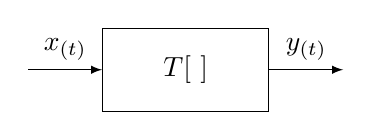
\begin{tikzpicture}[
            node distance=2cm,
            >=latex
            ]

            \node [coordinate] (input) {};
            \node [draw, rectangle,right of = input, minimum height=3em, minimum width=6em] (block) {$T[\ ]$};
            \node [coordinate, right of = block] (output) {};
            
            \draw[draw,->] (input) -- node[above]{$x_{(t)}$} (block);
            \draw[->] (block) -- node[above]{$y_{(t)}$} (output);
        \end{tikzpicture}    
    \label{Def sistema monodimensionale}
    \end{figure}
    Il sistema applica la trasformazione $T[\ ]: y_{(t)} = T[x_{(t)}]$ in gemerale \\ $y_{(t)} = T[x_{(\alpha)},t]$. 
    \subsection{Propietá dei Sistemi Lineari Tempo Invarianti (LTI)}
        \begin{itemize}
            \item {Linearitá:
                \[
                    x_{(t)} = ax_{1(t)}+bx_{2(t)} \overset{T[\ ]}{\Rightarrow} y_{(t)} = aT[x_{1(t)}]+b T[x_{2(t)}]
                \]
                Oppure separando la variabile del tempo:
                \[
                    x_{(t)} = ax_{1(t)}+bx_{2(t)} \overset{T[\ ]}{\Rightarrow} y_{(t)} = aT[x_{1(\alpha)},t]+b T[x_{2(\alpha)},t]
                \]
                É il principio di linearitá o sovrapposizione degli effetti visto a elettrotecnica.
            }\label{SM Linearita}
            \item {Stazionarietá:
                \[
                    y_{(t)} = T[x_{(t)}] \rightarrow y_{(t-t_0)} = T[x_{(t-t_0)}]  
                \]
            }\label{SM Stazionarieta}
            \item {Causalitá:
                \[
                    y_{(t)} = T[x_{(\alpha)},\alpha\leq t]
                \]
                L'uscita all'istante $t$ dipende dall'ingresso ad instanti precedenti o al piú uguali a $t$, si basa su valori precendenti a 
                $t$ non puó prevedere il futuro. Ne derivano 2 distinzioni di trasformazioni:
                \begin{itemize}
                    \item Real Time: necessariamente causale (é nel presente)
                    \item Virtual time: Causale o Non Causale (es. ho tutto un file al quale posso prevedere i bit o frame successivi per applicarne un post-processing)
                \end{itemize}
            }\label{SM Causalita}
            \item {Stabilitá BIBO:
                Se il segnale $x_{(t)}$ ha ampiezza limitata $\rightarrow$ l'uscita ha ampiezza limitata:
                    \[
                        |x_{(t)}|\leq M \rightarrow |y_{(t)}|\leq K 
                    \]
            }\label{SM Stabilita BIBO}
            \item {Invertibilitá:
                \[
                    y_{(t)} = T[x_{(\alpha)},t] \overset{\text{Se} \exists}{\Rightarrow} x_{(t)} = T^{-1}[y_{(\alpha)},t]
                \]
            }\label{SM Invertibilita}
            \item {Memoria:
                Un sistema é:
                \begin{itemize}
                    \item {Senza memoria: se $y_{(t)} = T[x_{(\alpha)},\alpha=t]$}
                    \item {Con Memoria: $y_{(t)} =\int_{-\infty}^{t}x_{(\alpha)} d\alpha$ l'uscita all'istante $t$ dipende anche da valori dell'ingresso 
                          ad istanti diversi da $t$. Nota bene é l'integrale di convoluzione di $x_{(t)} \otimes u_{(t)}$ 
                    }
                \end{itemize}
            }\label{SM Memoria}
        \end{itemize}
    \subsection{Propietá dei Sistemi Lineari Stazionari (SLS)}
        Sono sistemi che godono delle propietá di Linearitá \ref{SM Linearita} e di Stazionarietá \ref*{SM Stazionarieta}:
        \begin{figure}[H]
            \centering 
            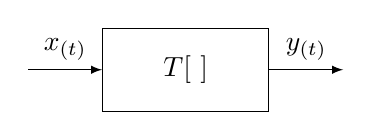
\begin{tikzpicture}[
                node distance=2cm,
                >=latex
                ]

                \node [coordinate] (input) {};
                \node [draw, rectangle,right of = input, minimum height=3em, minimum width=6em] (block) {$T[\ ]$};
                \node [coordinate, right of = block] (output) {};
                
                \draw[draw,->] (input) -- node[above]{$x_{(t)}$} (block);
                \draw[->] (block) -- node[above]{$y_{(t)}$} (output);
            \end{tikzpicture}    
        \label{Def SLS}
        \end{figure}  
        Troviamo la relazione tra ingresso e uscita:
        \begin{align}
            y_{(t)} &= T[x_{(\alpha)},t] =T[x_{(t)}] = T[x_{(t)} \otimes \delta_{(t)}] = T[\int_{-\infty}^{\infty}x_{(\alpha)}\delta_{(t-\alpha)}d\alpha]\nonumber \\        
                    &\overset{\ref*{SM Linearita}}{\Rightarrow} \underset{(\alpha)}{\int_{-\infty}^{\infty}}\underset{(t)}{T}[x_{(\alpha)}\delta_{(t-\alpha)}]d\alpha =\underset{(\alpha)}{\int_{-\infty}^{\infty}}x_{(\alpha)}\underset{(t)}{T}[\delta_{(t-\alpha)}]d\alpha\nonumber         
        \end{align}  
        Definiamo la trasformata nota del $\delta_{(t)}$:
        \begin{figure}[H]
            \centering 
            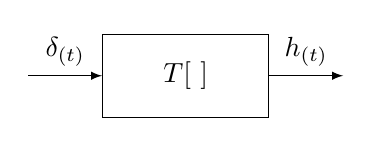
\begin{tikzpicture}[
                node distance=2cm,
                >=latex
                ]

                \node [coordinate] (input) {};
                \node [draw, rectangle,right of = input, minimum height=3em, minimum width=6em] (block) {$T[\ ]$};
                \node [coordinate, right of = block] (output) {};
                
                \draw[draw,->] (input) -- node[above]{$\delta_{(t)}$} (block);
                \draw[->] (block) -- node[above]{$h_{(t)}$} (output);
            \end{tikzpicture}    
        \label{Def impulso}
        \end{figure}
        Sollecitando il sistema con una Delta di Dirac ho la sua risposta impulsiva\index{Risposta Impulsiva}. Nel caso dei sistemi $SLS$ l'impulso
        in uscita caratterizza completamente il sistema. Nel nostro caso $T[\delta_{(t-\alpha)}]$ non é altro che una traslazione della $T[\delta_{(t)}]$ per la 
        Stazionarietá \ref*{SM Stazionarieta}: 
        \[
            y_{(t)} =\int_{-\infty}^{\infty}x_{(\alpha)}h_{(t-\alpha)}d\alpha = x_{(t)}\otimes h_{(t)} 
        \]
        La trasformata del sistema dipende solo dalla $h_{(t)}$ (risposta impulsiva del sistema)\index{Risposta Impulsiva}. Passando al dominio della frequenza per la propietá della convoluzione \ref{Convoluzione}:
        \[
            Y_{(f)} =X_{(f)}\otimes H_{(f)} 
        \]
        Dove $H_{(f)} = TCF[h_{(t)}] = \int_{-\infty}^{\infty} h_{(t)}e^{-j2\pi ft}$ é la risposta in frequenza del sistema $SLS$. Esistono vari modi
        per calcolare $h_{(t)}$:
        \begin{itemize}
            \item {
                Utilizzando un impulso di Dirac e le sue propietá, ma l'impulso di dirac é difficile da realizzare. 
            }
            \item {
                Calcolo $H_{(f)}$ mandanndo in ingresso un segnale del quale sia nota la sua risposta e calcolo il rapporto uscita/ingresso 
                $H_{(f)} = \frac{Y_{(f)}}{X_{(f)}}$
            }
            \item {
                Mandanndo in ingresso un esponenziale:
                \[
                    y_{(t)} = x_{(t)}\otimes h_{(t)},\ x_{(t)} = e^{j2\pi f_0t}
                \]
                \begin{align}
                    y_{(t)} &= \int_{-\infty}^{\infty}x_{(t-\alpha)}h_{(t)}d\alpha = \int_{-\infty}^{\infty}h_{(\alpha)} e^{j2\pi f_0(t-\alpha)}d\alpha \nonumber \\
                            &= e^{j2\pi f_0t}\int_{-\infty}^{\infty}h_{(\alpha)} e^{j2\pi f_0\alpha}d\alpha = x_{(t)}H_{(f_0)} \nonumber 
                \end{align}
                \[
                    H_{(f_0)} = \frac{y_{(t)}}{x_{(t)}}
                \]  
                Posso calcolare la risposta in $f_0$, posso variare la frequenza e calcolare $H_{(f)} = \eval*{\frac{y_{(t)}}{x_{(t)}}}_{x_{(t)} = e^{j2\pi ft}}$
            }
        \end{itemize}
        \subsubsection{Risposta in frequenza}
            La risposta in frequenza $H_{(f)} \in \mathbb{C}$:
            \[
                H_{(f)} = |H_{(f)}| e^{j\angle H_{(f)} }
            \]  
            \begin{itemize}
                \item$|H_{(f)}|$: Risposta in ampiezza
                \item $\angle H_{(f)}$: Risposta in fase 
            \end{itemize}
            \[
                Y_{(f)} = X_{(f)} H_{(f)} = 
                \begin{cases}
                    |Y_{(f)}| &= |X_{(f)}||H_{(f)}| \nonumber \\
                    \angle Y_{(f)} &= \angle X_{(f)} + \angle H_{(f)} \nonumber
                \end{cases} 
            \]  
        \subsubsection{Sistemi in cascata e in parallelo}
            \begin{itemize}
                \item {Sistemi in cascata:
                    \begin{figure}[H]
                        \centering
                        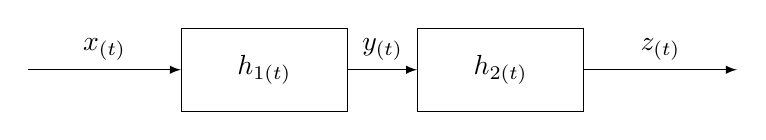
\begin{tikzpicture}[
                            node distance=3cm,
                            >=latex
                            ]
            
                            \node [coordinate] (input) {};
                            \node [draw, rectangle,right of = input, minimum height=3em, minimum width=6em] (sis1) {$h_{1(t)}$};
                            \node [draw, rectangle,right of = sis1, minimum height=3em, minimum width=6em] (sis2) {$h_{2(t)}$};
                            \node [coordinate, right of = sis2] (output) {};
                            
                            \draw[draw,->] (input) -- node[above]{$x_{(t)}$} (sis1);
                            \draw[draw,->] (sis1) -- node[above]{$y_{(t)}$} (sis2);
                            \draw[->] (sis2) -- node[above]{$z_{(t)}$} (output);
                        \end{tikzpicture}
                        \caption{sistemi in cascata}
                        \label{fig:sistemi in cascata}
                    \end{figure}    
                    \begin{figure}[H]
                        \centering
                        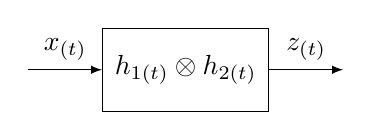
\begin{tikzpicture}[
                            node distance=2cm,
                            >=latex
                            ]
            
                            \node [coordinate] (input) {};
                            \node [draw, rectangle,right of = input, minimum height=3em, minimum width=6em] (block) {$h_{1(t)}\otimes h_{2(t)}$};
                            \node [coordinate, right of = block] (output) {};
                            
                            \draw[draw,->] (input) -- node[above]{$x_{(t)}$} (block);
                            \draw[->] (block) -- node[above]{$z_{(t)}$} (output);
                        \end{tikzpicture}
                        \caption{equivalente sistemi in cascata}
                        \label{fig:equivalente sistemi in cascata}
                    \end{figure}
                    \begin{align}
                        y_{(t)} &= x_{(t)}\otimes h_{1(t)} \nonumber \\
                        z_{(t)} &= y_{(t)}\otimes h_{2(t)} = [x_{(t)}\otimes h_{1(t)}]\otimes h_{2(t)} = x_{(t)}\otimes h_{1(t)}\otimes h_{2(t)}  \nonumber \\
                        z_{(t)} &= x_{(t)}\otimes h_{(t)}  \nonumber 
                    \end{align}
                    \[
                        \text{Risposta Impulsiva}: h_{(t)} = h_{1(t)}\otimes h_{2(t)}
                    \]
                    \[
                        \text{Risposta in Frequenza}: H_{(f)} = H_{1(f)} H_{2(f)}
                    \]
                }
                \item {Sistemi in parallelo:
                    \begin{figure}[H]
                        \centering
                        \begin{tikzpicture}[
                            node distance=2cm,
                            >=latex
                            ]
            
                            \node [coordinate] (input) {};
                            
                            \node [coordinate, right of = input] (node1) {};
                            \node [coordinate, above of = node1] (node2) {};
                            \node [coordinate, below of = node1] (node3) {};
                            
                            \node [draw, rectangle,right of = node2, minimum height=3em, minimum width=6em] (sis1) {$h_{1(t)}$};
                            \node [draw, rectangle,right of = node3, minimum height=3em, minimum width=6em] (sis2) {$h_{2(t)}$};
                            
                            \node [coordinate, right of = sis1] (node4) {};
                            \node [coordinate, right of = sis2] (node5) {};
                            \node [draw,circle, above of = node5] (node6) {$+$};
                            
                            \node [coordinate, right of = node6] (output) {};

                            \draw[draw,->] (input) -- node[above]{$x_{(t)}$}(node1);
                            \draw[draw,-] (node1) -- (node2);
                            \draw[draw,-] (node1) -- (node3);
                            \draw[draw,-] (node2) -- (sis1);
                            \draw[draw,-] (node3) -- (sis2);
                            \draw[draw,-] (sis1) -- node[above]{$y_{1(t)}$}(node4);
                            \draw[draw,-] (sis2) -- node[above]{$y_{2(t)}$}(node5);
                            \draw[draw,-] (node4) -- (node6);
                            \draw[draw,-] (node5) -- (node6);
                            \draw[draw,->] (node6) -- node[above]{$y_{(t)}$} (output);

                        \end{tikzpicture}
                        \caption{sistemi in cascata}
                        \label{fig:sistemi in parallelo}
                    \end{figure}    
                    \begin{figure}[H]
                        \centering
                        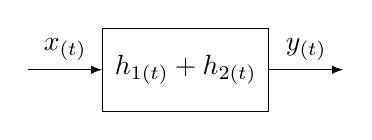
\begin{tikzpicture}[
                            node distance=2cm,
                            >=latex
                            ]
            
                            \node [coordinate] (input) {};
                            \node [draw, rectangle,right of = input, minimum height=3em, minimum width=6em] (block) {$h_{1(t)}+h_{2(t)}$};
                            \node [coordinate, right of = block] (output) {};
                            
                            \draw[draw,->] (input) -- node[above]{$x_{(t)}$} (block);
                            \draw[->] (block) -- node[above]{$y_{(t)}$} (output);
                        \end{tikzpicture}
                        \caption{equivalente sistemi in parallelo}
                        \label{fig:equivalente sistemi in parallelo}
                    \end{figure}
                    \begin{align}
                        y_{(t)} &= y_{1(t)}\otimes y_{2(t)} = x_{(t)}\otimes h_{1(t)} + x_{(t)}\otimes h_{2(t)} \nonumber \\
                                &= x_{(t)}\otimes[h_{1(t)}+h_{2(t)}] = x_{(t)}\otimes h_{(t)}\nonumber 
                    \end{align}
                    \[
                        \text{Risposta Impulsiva}: h_{(t)} = h_{1(t)}+h_{2(t)}
                    \]
                    \[
                        \text{Risposta in Frequenza}: H_{(f)} = H_{1(f)} + H_{2(f)}
                    \]
                }
            \end{itemize}
        
    \subsection{Risposta di un sistema causale e risposta impulsiva}
        \begin{figure}[H]
            \centering
            \begin{tikzpicture}
                \begin{axis}[
                xlabel={$t$},
                ylabel={$h_{(t)}$},
                xmin=-2.5, xmax=5,
                ymin=-2, ymax=5,
                axis lines=middle,
                axis line style={->},
                width = 10cm,
                height = 6cm
                ]
                \addplot[blue, domain=0:5,thick, samples=100] {1.5+sin(deg(x)) + cos(deg(2*x))};
                \addplot[const plot,blue,thick] coordinates{(-5,0)(0,0)(0,2.5)};
                \end{axis}
            \end{tikzpicture}
            \caption{Risposta impulsiva di un sistema}
            \label{fig:Risposta impulsiva di un sistema}
        \end{figure}
        $h_{(t)} = h_{(t)} \dotproduct u_{(t)}$ 
        \begin{align}
            y_{(t)} &= x_{(t)} \otimes h_{(t)} = \int_{-\infty}^{\infty}x_{(\alpha)}h_{(t-\alpha)} d\alpha = \int_{-\infty}^{\infty}x_{(\alpha)}h_{(t-\alpha)}u_{(t-\alpha)} d\alpha \nonumber \\
                    &= \int_{-\infty}^{t}x_{(\alpha)}h_{(t-\alpha)} d\alpha 
        \end{align}
        giungiamo all'integrale che definisce la Causalitá \ref{SM Causalita}: un sistema é causale se la sua risposta impulsiva 
        é solo definita per $t>0$.
        \begin{figure}[H]
            \centering
            \begin{tikzpicture}
                \begin{axis}[
                xlabel={$t$},
                ylabel={$h_{(t)}$},
                xmin=-2.5, xmax=5,
                ymin=-2, ymax=5,
                axis lines=middle,
                axis line style={->},
                width = 10cm,
                height = 6cm
                ]
                \addplot[blue, domain=-5:3,thick, samples=100] {1.5-sin(deg(x)) - cos(deg(2*x))};
                \addplot[const plot,blue,thick] coordinates{(5,0)(3,0)(3,0.4)};
                \end{axis}
            \end{tikzpicture}
            \caption{Uscita di un sisetma causale}
            \label{fig:Risposta impulsiva di un sistema causale}
        \end{figure}
        Dal valore $3$ in poi la risposta impulsiva rende il sistema causale.
    
        \subsubsection{Stabilitá BIBO su $h_{(t)}$}
            \begin{align}
                |y_{(t)}| &= \left|\int_{-\infty}^{\infty}x_{(\alpha)}h_{(t-\alpha)} d\alpha \right|\leq \int_{-\infty}^{\infty}|x_{(\alpha)}||h_{(t-\alpha)}| d\alpha \nonumber \\
                          &\leq M\left|\int_{-\infty}^{\infty}h_{(t-\alpha)} d\alpha \right| <K\nonumber
            \end{align}
            Se l'ingresso $y<M$ allora lo é anche l'uscita. Ne deriva la C.S(Condizione Sufficiente): Assoluta integrabilitá della $h_{(t)}$ \index{Assoluta integrabilitá $h_{(t)}$},
            se il sistema é bounded anche l'integrale deve esserlo.RICONTROLLA
            TROVA L CONDIZIONE NECESSARIA SUL LIBRO.
    \subsection{Filtri Ideali}
        \paragraph{Banda di un segnale} É la porzione di spettro calcolata sul semiasse positivo delle
        frequenze dove lo spettro é diverso da zero.
        \[
            B = {f\dotproduct H_{(f)} \neq 0, f >0}  
        \]
        \subsubsection{Filtro Passa Basso di banda B - Low Pass Filter (LP)}\label{Filtro Passa Basso di banda B - Low Pass Filter (LP)}
            \begin{figure}[H]
                \centering

                \begin{tikzpicture}
                    \begin{axis}[
                        domain=-5:5,
                        samples=200,
                        axis lines=middle,
                        xlabel=$f$,
                        ylabel=$H_{LP(f)}$,
                        xmax=5,
                        xmin=-5,
                        ymin=-0.3,
                        ymax=2.5,
                        xtick={-2,2},
                        xticklabels={$-B$,$B$},
                        ytick={},
                        yticklabels={},
                        width=9cm,
                        height=6cm
                    ]
                    \addplot [const plot,thick,orange] coordinates{(-5,0)(-2,0)};
                    \addplot [const plot,thick,orange] coordinates{(5,0)(2,0)};
                    \addplot [const plot,thick,orange] coordinates{(-2,0)(-2,1)};
                    \addplot [const plot,thick,orange] coordinates{(-2,1)(2,1)};
                    \addplot [const plot,thick,orange] coordinates{(2,1)(2,0)};
                    
                    \end{axis}
                \end{tikzpicture}

                \caption{Filtro passa basso ideale: Risposta in frequenza}
                \label{fig:filtro passa basso ideale}
            \end{figure} 
            
            \paragraph{Risposta in frequenza:}
            \[
                H_{LP(f)}\triangleq rect\left(\frac{f}{2B}\right)  
            \]
            \paragraph{Risposta impulsiva:}
            \[
                h_{LP(t)}\triangleq 2Bsinc(2Bt)  
            \]
            La risposta impulsiva non é causale, ma posso troncarla e spostarna nel semiasse positivo per renderlo tale, ma non é piú ideale:
            \begin{figure}[H]
                \centering

                \begin{tikzpicture}
                    \begin{axis}[
                        domain=-0.3:10,
                        samples=200,
                        axis lines=middle,
                        xlabel=$t$,
                        ylabel=$h_{LP(t)}$,
                        xmax=10,
                        xmin=-1,
                        ymin=-0.3,
                        ymax=1.5,
                        xtick={},
                        xticklabels={},
                        ytick={},
                        yticklabels={},
                        width=8cm
                    ]
                    \addplot [const plot,thick,orange, domain = 0:8, samples = 1000] {(sin(deg((x-4)*10*pi))/((x-4)*10*pi))};
                    \end{axis}
                \end{tikzpicture}

                \caption{Filtro passa basso causale: risposta impulsiva}
                \label{fig:filtro passa basso ideale causale}
            \end{figure} 

            \paragraph{Cricuito Filtro Passa Basso:}
            
            \begin{figure}[H]
                \centering
                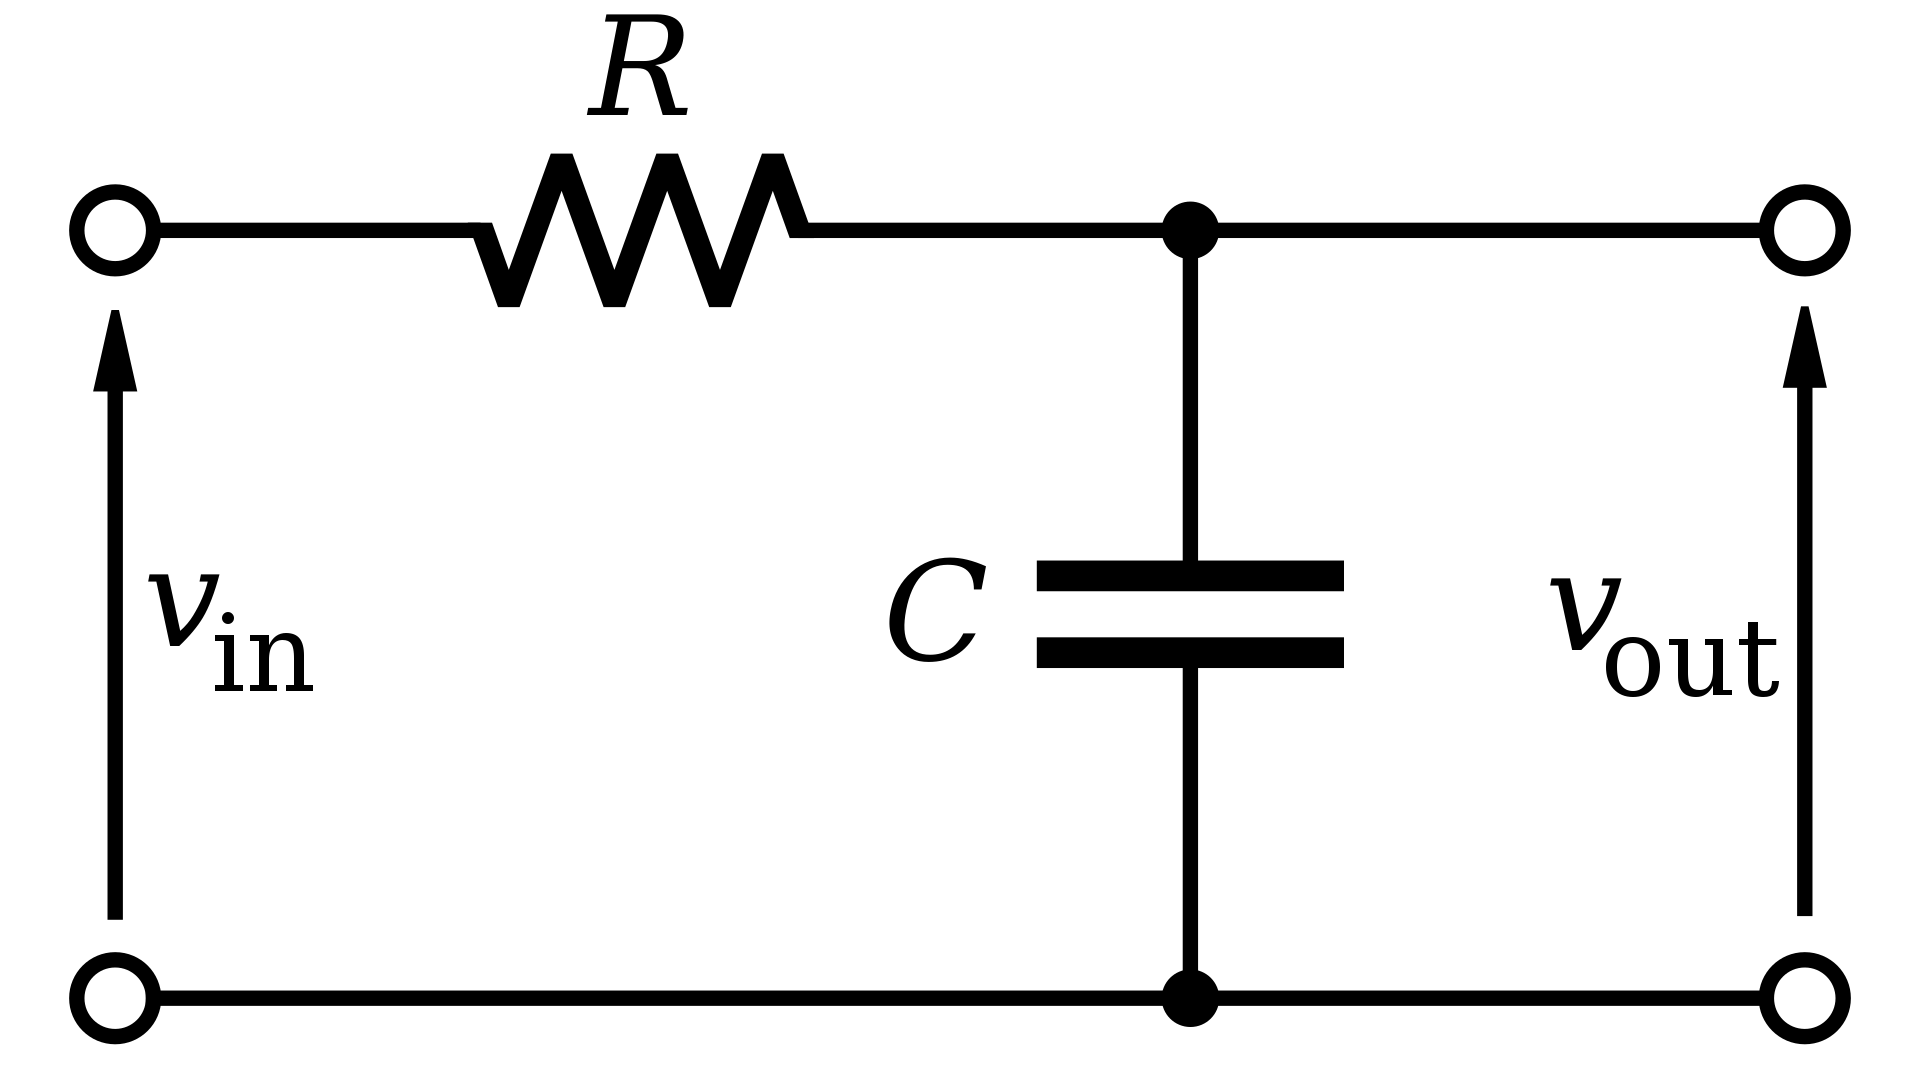
\includegraphics[width=4cm]{media/1st_Order_Lowpass_Filter_RC.png}
                \caption{Circuito filtro passa basso ideale}
                \label{fig:circuito filtro passa basso ideale}
            \end{figure}
            \[
                \frac{V_{out}}{V_{in}} = H_{(f)} = \frac{1}{1+j\frac{f}{f_T}},\ f_T = \frac{1}{2\pi RC}
            \] 
            Possiamo rappresentare in sacala logaritmica il filtro: $\eval*{|H_{(f)}|}_{db} = 10log\left( \frac{\left|H_{(f)}\right|^2}{\left|H_{(f_0)}\right|^2} \right)$.
            Prendiamo la frequenza di riferimento $f_0: H_{(f_0)} = 1$
            \begin{figure}[H]
                \centering
                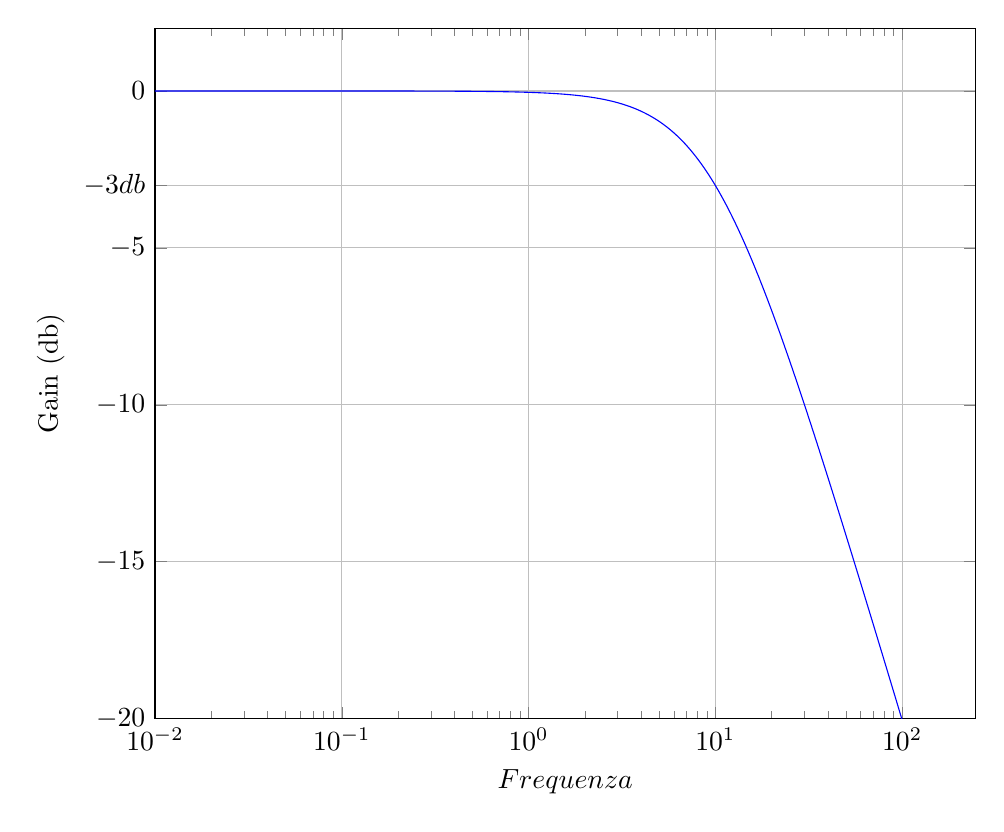
\begin{tikzpicture}
                    \begin{semilogxaxis}[
                        width=12cm,
                        xmin=0.01,
                        ymin=-20,
                        xmajorgrids=true,
                        ymajorgrids=true,
                        xlabel=$Frequenza$,
                        ylabel={Gain (db)},
                        ytick={0,-3,-5,-10,-15,-20},
                        yticklabels={$0$,$-3db$,$-5$,$-10$,$-15$,$-20$}
                    ] 
                        \addplot[domain=0.01:10000,samples=1000,color=blue]{20*log10(1/sqrt(1+(x/10)^2))};
                    \end{semilogxaxis}
                \end{tikzpicture}
                \caption{Filtro passa basso ideale in scala logaritmica}
                \label{fig:LP filter logartithm}
            \end{figure} 
            
            Otteniamo la Frequenza di taglio \index{Frequenza di taglio}$f_T$ all'ampiezza di $-3db$, in questo caso $f_T = 10$, alla quale
            il filtro "taglia" o meglio riduce tutte le ampiezze in ingresso verso lo 0.

            RIGUARDA SUL LIBRO FORMULA PER IL CALCOLO DI 1/2 PER IL MODULO DI Hf e le formule di risposta dei circuiti, mhh la fase?
            \begin{figure}[H]
                \centering
                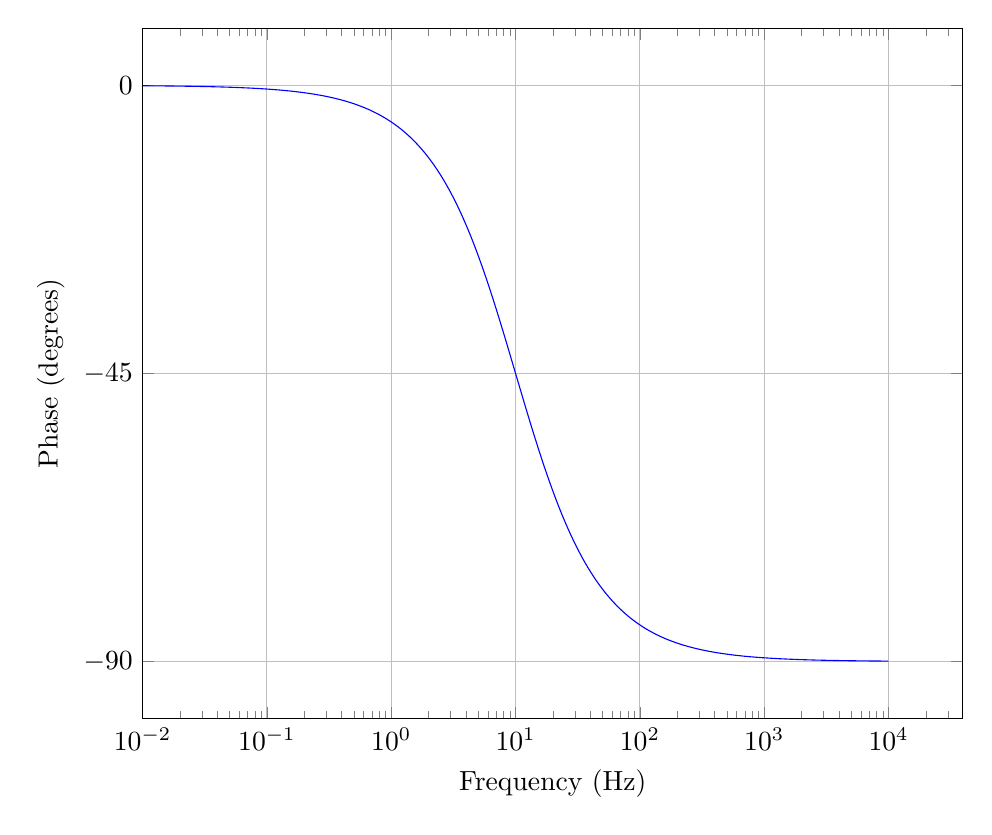
\begin{tikzpicture}
                    \begin{semilogxaxis}[
                        width=12cm,
                        xmin = 0.01,
                        xmajorgrids=true,
                        ymajorgrids=true,
                        xlabel={Frequency (Hz)},
                        ylabel={Phase (degrees)},
                        ytick={-180,-135,-90,-45,0,45,90,135,180},
                        yticklabels={$-180$,$-135$,$-90$,$-45$,$0$,$45$,$90$,$135$,$180$}
                    ] 
                        \addplot[domain=0.01:10000,samples=1000,color=blue]{(atan(-x/10))};
                    \end{semilogxaxis}
                \end{tikzpicture}
                \caption{Filtro passa basso ideale fase}
                \label{fig:LP filter phase}
            \end{figure} 

            $Osservazione$: 
            \begin{itemize}
                \item{
                    Al tendere di $B$ a $0$ il valore che il filtro fa passare é il valor medio del segnale, tanto da tendere
                    a un filtro $LP$ con spettro $\delta_{(t)}$, ma é difficilmente realizzabile.
                }
                \item{
                    La banda di un filtro é quanto si estende da $0 \rightarrow f^+$ fino a arrivare a $B$,$[0,B]$
                }
                \item{
                    Se il filtro é un filtro $BP$ la banda é l'ampiezza della banda che lascia passare $[f_0-B,f_0+B] = B$
                }
            \end{itemize}
        \subsubsection{Filtro Passa Alto di banda B - High Pass Filter (HP)}\label{Filtro Passa Alto di banda B - High Pass Filter (HP)}
            \begin{figure}[H]
                \centering
                \begin{tikzpicture}
                    \begin{axis}[
                        domain=-5:5,
                        samples=200,
                        axis lines=middle,
                        xlabel=$f$,
                        ylabel=$H_{HP(f)}$,
                        xmax=5,
                        xmin=-5,
                        ymin=-0.3,
                        ymax=2.5,
                        xtick={-2,2},
                        xticklabels={$-B$,$B$},
                        ytick={},
                        yticklabels={},
                        width=9cm,
                        height=6cm
                    ]
                    \addplot [const plot,thick,orange] coordinates{(-5,1)(-2,1)};
                    \addplot [const plot,thick,orange] coordinates{(5,1)(2,1)};
                    \addplot [const plot,thick,orange] coordinates{(-2,0)(-2,1)};
                    \addplot [const plot,thick,orange] coordinates{(-2,0)(2,0)};
                    \addplot [const plot,thick,orange] coordinates{(2,1)(2,0)};
                    
                    \end{axis}
                \end{tikzpicture}

                \caption{Filtro passa alto ideale: Risposta in frequenza}
                \label{fig:filtro passa alto ideale}
            \end{figure}  
            
            \paragraph{Risposta in frequenza:}
            \[
                H_{HP(f)}\triangleq 1 - rect\left(\frac{f}{2B}\right)  
            \]
            \paragraph{Risposta impulsiva:}
            \[
                h_{HP(t)}\triangleq \delta_{(t)} - 2Bsinc(2Bt)  
            \]

        \paragraph{Cricuito Filtro Passa Alto:}
            \begin{figure}[H]
                \centering
                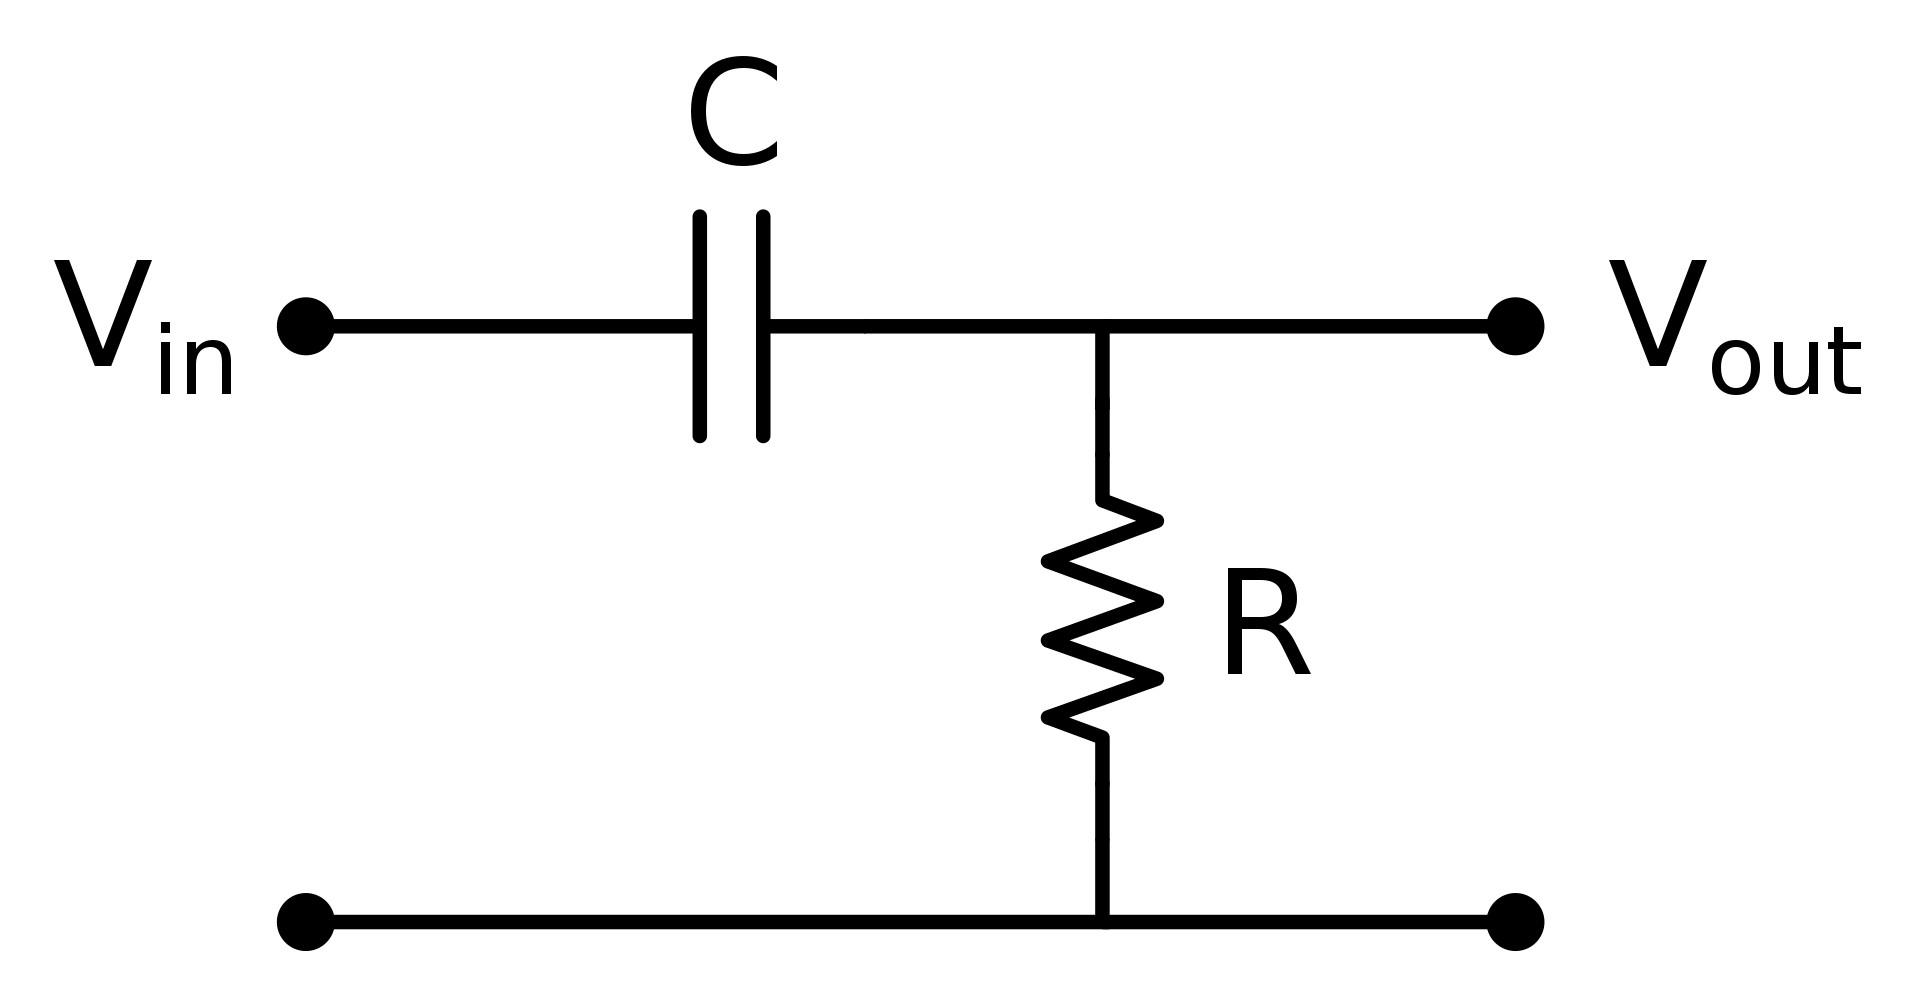
\includegraphics[width=4cm]{media/CR_high_pass_filter.png}
                \caption{Circuito filtro passa alto ideale}
                \label{fig:circuito filtro passa alto ideale}
            \end{figure}
            \[
                    H_{(f)} = \frac{fRC}{1+fRC}  
            \] 
        In scala logaritmica:
        \begin{figure}[H]
            \centering
            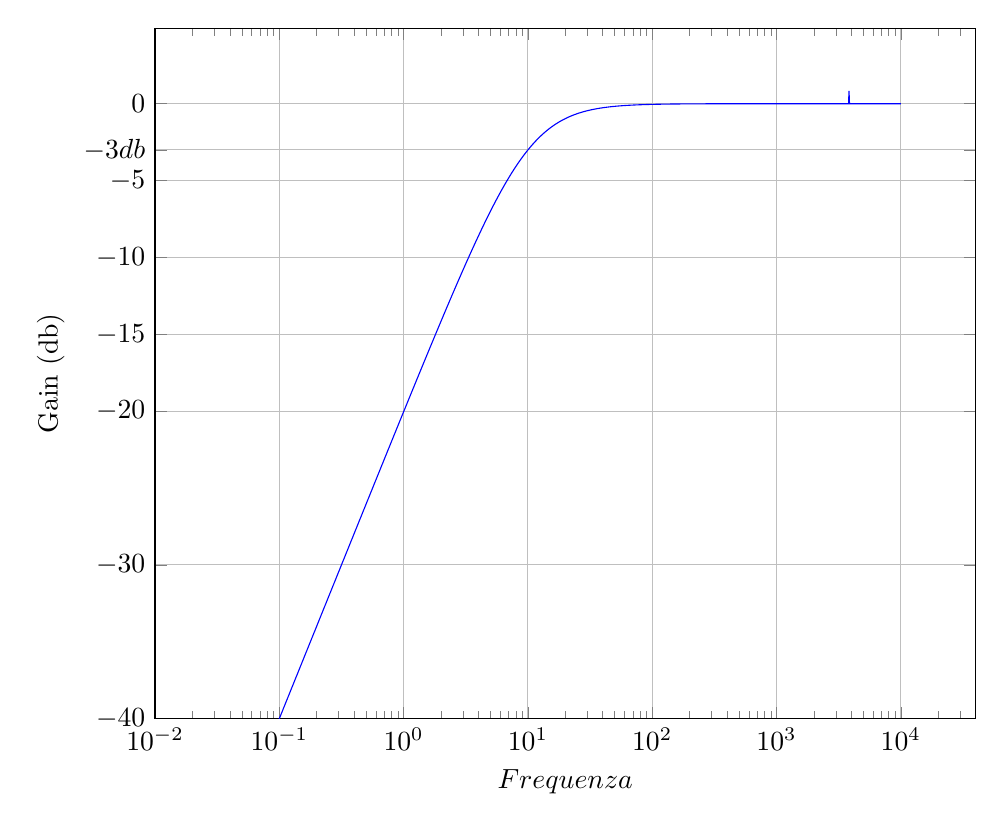
\begin{tikzpicture}
                \begin{semilogxaxis}[
                    width=12cm,
                    xmin=0.01,
                    ymin=-40,
                    xmajorgrids=true,
                    ymajorgrids=true,
                    xlabel=$Frequenza$,
                    ylabel={Gain (db)},
                    ytick={0,-3,-5,-10,-15,-20,-30,-40},
                    yticklabels={$0$,$-3db$,$-5$,$-10$,$-15$,$-20$,$-30$,$-40$}
                ] 
                    \addplot[domain=0.01:10000,samples=1500,color=blue]{20*log10(sqrt((x/10)^2)/sqrt(1+(x/10)^2))};
                \end{semilogxaxis}
            \end{tikzpicture}
            \caption{Filtro passa alto ideale in scala logaritmica}
            \label{fig:HP filter logartithm}
        \end{figure} 
        \begin{figure}[H]
            \centering
            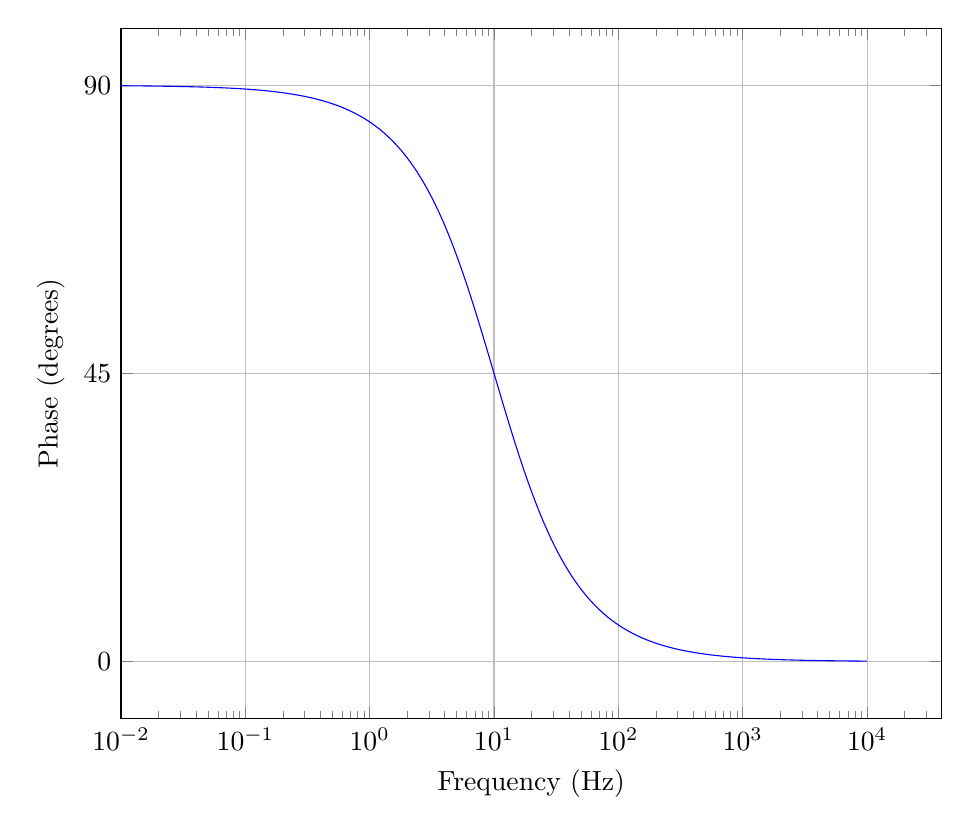
\begin{tikzpicture}
                \begin{semilogxaxis}[
                    width=12cm,
                    xmin = 0.01,
                    xmajorgrids=true,
                    ymajorgrids=true,
                    xlabel={Frequency (Hz)},
                    ylabel={Phase (degrees)},
                    ytick={-180,-135,-90,-45,0,45,90,135,180},
                    yticklabels={$-180$,$-135$,$-90$,$-45$,$0$,$45$,$90$,$135$,$180$}
                ] 
                    \addplot[domain=0.01:10000,samples=1000,color=blue]{(atan(-x/10)+90)};
                \end{semilogxaxis}
            \end{tikzpicture}
            \caption{Filtro passa alto ideale fase}
            \label{fig:HP filter phase}
        \end{figure} 
        Si nota come avendo preso la $f_T$ corrisponde a $RC = 10$. 
        \subsubsection{Filtro Passa Banda di banda B - Band Pass Filter (BP)}\label{Filtro Passa Banda di banda B - Band Pass Filter (BP)}
            \begin{figure}[H]
                \centering
                \begin{tikzpicture}
                    \begin{axis}[
                        domain=-5:5,
                        samples=200,
                        axis lines=middle,
                        xlabel=$f$,
                        ylabel=$H_{BP(f)}$,
                        xmax=5,
                        xmin=-5,
                        ymin=-0.3,
                        ymax=1.5,
                        xtick={-4,-3,-2,2,3,4},
                        xticklabels={$-B-f_0$,$-f_0$,$B-f_0$,$B+f_0$,$f_0$,$B+f_0$},
                        ytick={},
                        xticklabel style={font=\tiny},
                        yticklabels={},
                        width=12cm,
                        height=6cm
                    ]
                    \addplot [const plot,thick,orange] coordinates{(-5,0)(-4,0)};
                    \addplot [const plot,thick,orange] coordinates{(-2,0)(2,0)};
                    \addplot [const plot,thick,orange] coordinates{(5,0)(4,0)};
                    \addplot [const plot,thick,orange] coordinates{(-4,0)(-4,1)};

                    \addplot [const plot,thick,orange] coordinates{(-4,1)(-2,1)};
                    \addplot [const plot,thick,orange] coordinates{(-2,0)(-2,1)};
                    
                    \addplot [const plot,thick,orange] coordinates{(4,1)(2,1)};
                    \addplot [const plot,thick,orange] coordinates{(2,0)(2,1)};
                    \addplot [const plot,thick,orange] coordinates{(4,0)(4,1)};
                    
                    \end{axis}
                \end{tikzpicture}
                \caption{Filtro passa banda ideale: Risposta in frequenza}
                \label{fig:filtro passa banda ideale}
            \end{figure} 
            
            \paragraph{Risposta in frequenza:}
            \[
                H_{BP(f)}\triangleq H_{LP(f+f_0)} +H_{LP(f-f_0)} =  rect\left(\frac{f-f_0}{2B}\right) + rect\left(\frac{f+f_0}{2B}\right)  
            \]
            \paragraph{Risposta impulsiva:}
            \[
                h_{BP(t)}\triangleq 2Bsinc(2Bt) \cos(2\pi f_0t) = h_{LP(t)}\cos(2\pi f_0t)   
            \]
            \begin{figure}[H]
                \centering

                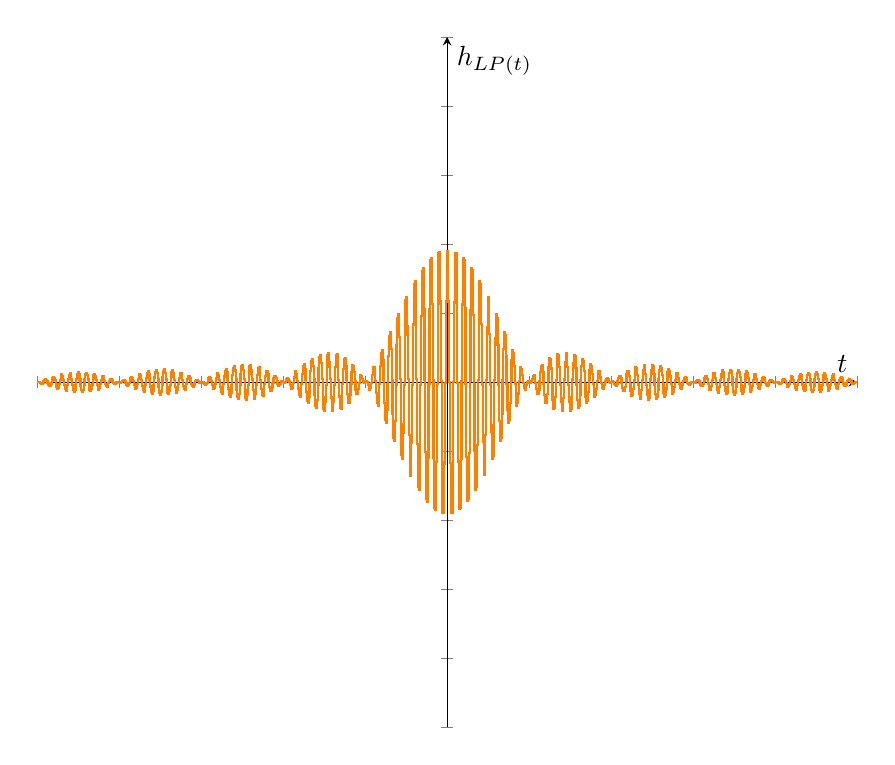
\begin{tikzpicture}
                    \begin{axis}[
                        domain=-5:5,
                        samples=200,
                        axis lines=middle,
                        xlabel=$t$,
                        ylabel=$h_{LP(t)}$,
                        xmax=5,
                        xmin=-5,
                        ymin=-5,
                        ymax=5,
                        xtick={},
                        xticklabels={},
                        ytick={},
                        yticklabels={},
                        width=12cm
                    ]
                    \addplot [const plot,thick,orange, samples = 1000] {(2*(sin(deg((x)*pi))/((x)*pi)))*cos(deg(2*pi*10*x))};
                    \end{axis}
                \end{tikzpicture}

                \caption{Filtro passa banda: risposta impulsiva}
                \label{fig:filtro passa banda ideale causale}
            \end{figure} 

            \paragraph{Cricuito Filtro Passa Banda:}
                \begin{figure}[H]
                    \centering
                    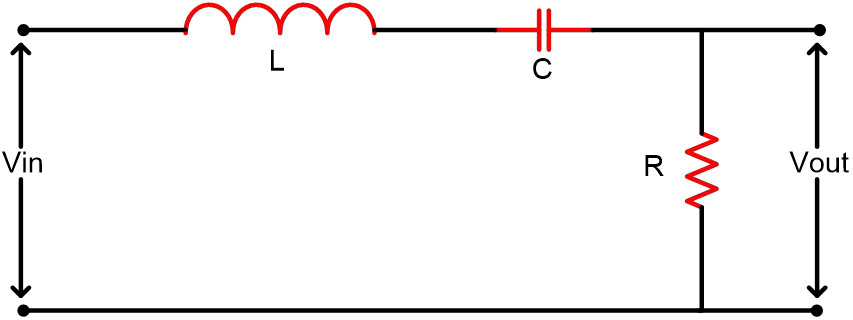
\includegraphics[width=4cm]{media/Band-Pass-Filter.png}
                    \caption{Circuito filtro passa banda ideale}
                    \label{fig:circuito filtro passa banda ideale}
                \end{figure} 
            In scala logaritmica:
            \begin{figure}[H]
                \centering
                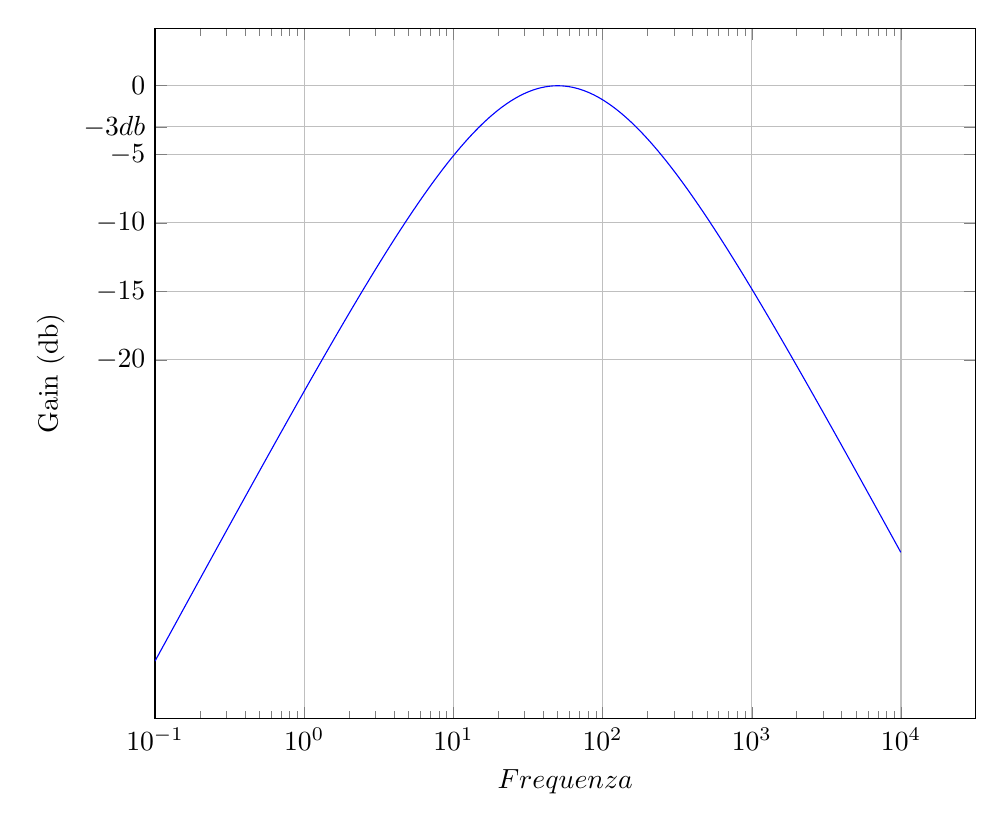
\begin{tikzpicture}
                    \begin{semilogxaxis}[
                        width=12cm,
                        xmin=10^-1,
                        xmajorgrids=true,
                        ymajorgrids=true,
                        xlabel=$Frequenza$,
                        ylabel={Gain (db)},
                        ytick={0,-3,-5,-10,-15,-20},
                        yticklabels={$0$,$-3db$,$-5$,$-10$,$-15$,$-20$}
                    ] 
                        \addplot[domain=10^-1:10000,samples=1000,color=blue]{20*log10(abs(((200*x)/(x^2+100*x+2500))))};
                    \end{semilogxaxis}
                \end{tikzpicture}
                \caption{Filtro passa banda ideale in scala logaritmica}
                \label{fig:BP filter logartithm}
            \end{figure}
            Non riesco a fare un grafico con pendenza maggiore ma é per capire che le frequenze sotto il valore di $-3db$
            vengono ridotte drasticamente.
            \begin{figure}[H]
                \centering
                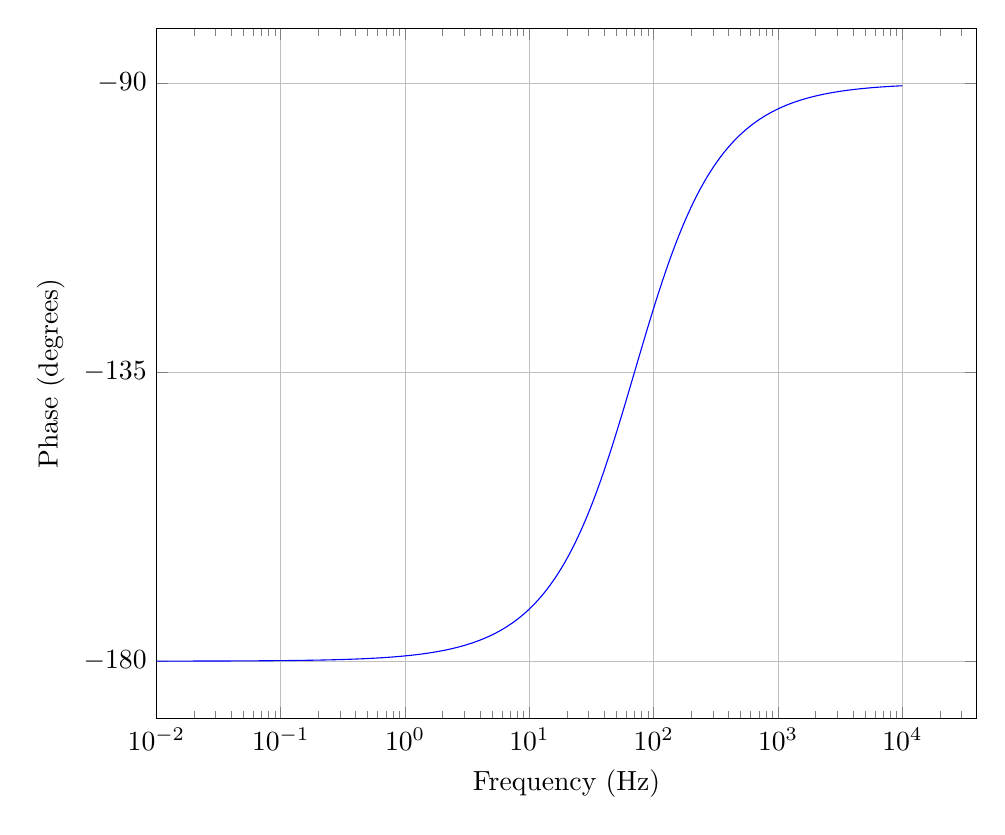
\begin{tikzpicture}
                    \begin{semilogxaxis}[
                        width=12cm,
                        xmin = 0.01,
                        xmajorgrids=true,
                        ymajorgrids=true,
                        xlabel={Frequency (Hz)},
                        ylabel={Phase (degrees)},
                        ytick={-180,-135,-90,-45,0,45,90,135,180},
                        yticklabels={$-180$,$-135$,$-90$,$-45$,$0$,$45$,$90$,$135$,$180$}
                    ] 
                        \addplot[domain=0.01:10000,samples=1000,color=blue]{(atan((x)/70))-180};
                    \end{semilogxaxis}
                \end{tikzpicture}
                \caption{Filtro passa banda ideale fase}
                \label{fig:BP filter phase}
            \end{figure} 
        \subsubsection{Filtro Elimina Banda di banda B - Band Stop Filter (BS)}\label{Filtro Elimina Banda di banda B - Band Stop Filter (BS)}
            \begin{figure}[H]
                \centering
                
                \begin{tikzpicture}
                    \begin{axis}[
                        domain=-5:5,
                        samples=200,
                        axis lines=middle,
                        xlabel=$f$,
                        ylabel=$H_{BS(f)}$,
                        xmax=5,
                        xmin=-5,
                        ymin=-0.3,
                        ymax=2.5,
                        xtick={-4,-3,-2,2,3,4},
                        xticklabels={$-B-f_0$,$-f_0$,$B-f_0$,$B+f_0$,$f_0$,$B+f_0$},
                        xticklabel style={font=\tiny},
                        ytick={},
                        yticklabels={},
                        width=9cm,
                        height=6cm
                    ]
                    \addplot [const plot,thick,orange] coordinates{(-5,1)(-4,1)};
                    \addplot [const plot,thick,orange] coordinates{(-2,1)(2,1)};
                    \addplot [const plot,thick,orange] coordinates{(5,1)(4,1)};
                    \addplot [const plot,thick,orange] coordinates{(-4,0)(-4,1)};

                    \addplot [const plot,thick,orange] coordinates{(-4,0)(-2,0)};
                    \addplot [const plot,thick,orange] coordinates{(-2,0)(-2,1)};
                    
                    \addplot [const plot,thick,orange] coordinates{(4,0)(2,0)};
                    \addplot [const plot,thick,orange] coordinates{(2,0)(2,1)};
                    \addplot [const plot,thick,orange] coordinates{(4,0)(4,1)};
                    
                    \end{axis}
                \end{tikzpicture}
                \caption{Filtro elimina banda ideale}
                \label{fig:filtro elimina banda ideale}
            \end{figure} 

            \paragraph{Risposta in frequenza:}
            \[
                H_{BS(f)}\triangleq 1 -(H_{BP(f+f_0)} +H_{BP(f-f_0)}) = 1- \left[ rect\left(\frac{f-f_0}{2B}\right) + rect\left(\frac{f+f_0}{2B}\right)\right]  
            \]
            \paragraph{Risposta impulsiva:}
            \[
                h_{BS(t)}\triangleq \delta_{(t)} - h_{BP(t)} = \delta_{(t)} - 2Bsinc(2Bt) \cos(2\pi f_0t)
            \]

            \paragraph{Cricuito Filtro Elimina Banda:}
                \begin{figure}[H]
                    \centering
                    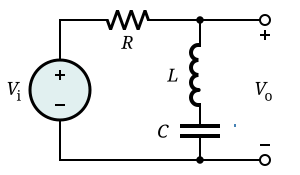
\includegraphics[width=4cm]{media/Band-Reject_Filter.png}
                    \caption{Circuito filtro elimina banda ideale}
                    \label{fig:circuito filtro elimina banda ideale}
                \end{figure}
                \[
                    H_{(f)} = \frac{}{}  
                \]
            In scala logaritmica:
            \begin{figure}[H]
                \centering
                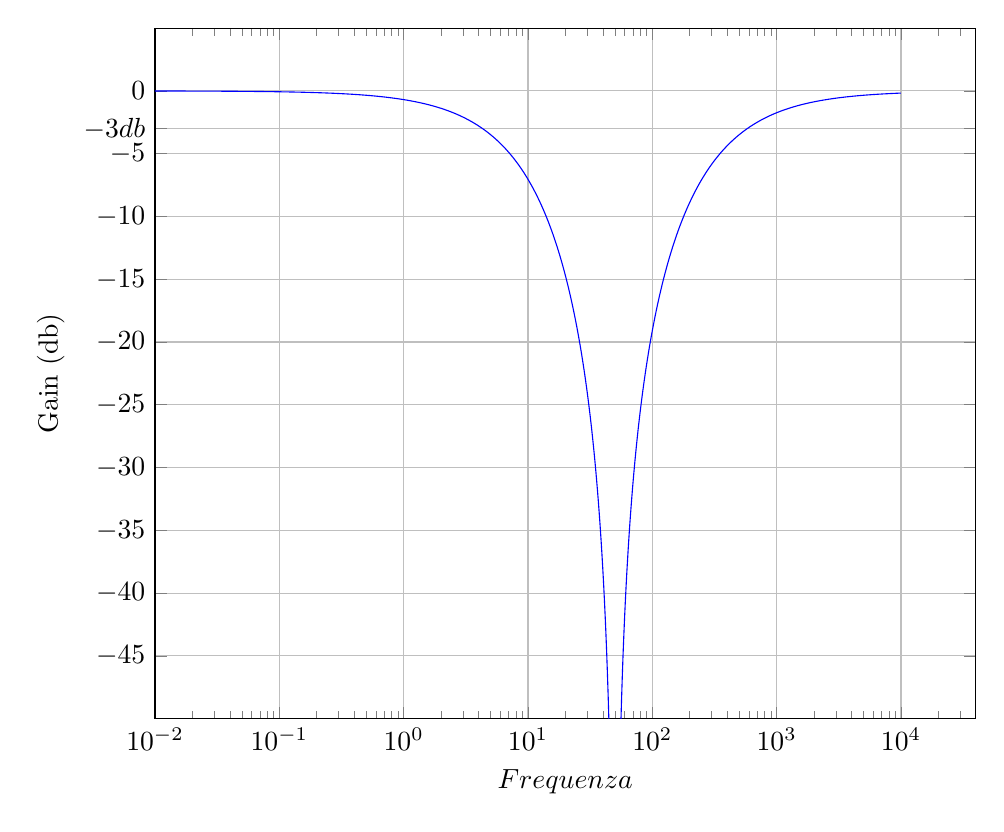
\begin{tikzpicture}
                    \begin{semilogxaxis}[
                        width=12cm,
                        xmin=0.01,
                        ymin=-50,
                        xmajorgrids=true,
                        ymajorgrids=true,
                        xlabel=$Frequenza$,
                        ylabel={Gain (db)},
                        ytick={0,-3,-5,-10,-15,-20,-25,-30,-35,-40,-45},
                        yticklabels={$0$,$-3db$,$-5$,$-10$,$-15$,$-20$,$-25$,$-30$,$-35$,$-40$,$-45$}
                    ] 
                        \addplot[domain=0.01:10000,samples=1000,color=blue]{20*log10(abs(1-((200*x)/(x^2+100*x+2500))))};
                    \end{semilogxaxis}
                \end{tikzpicture}
                \caption{Filtro elimina banda ideale in scala logaritmica}
                \label{fig:BS filter logartithm}
            \end{figure}
            \begin{figure}[H]
                \centering
                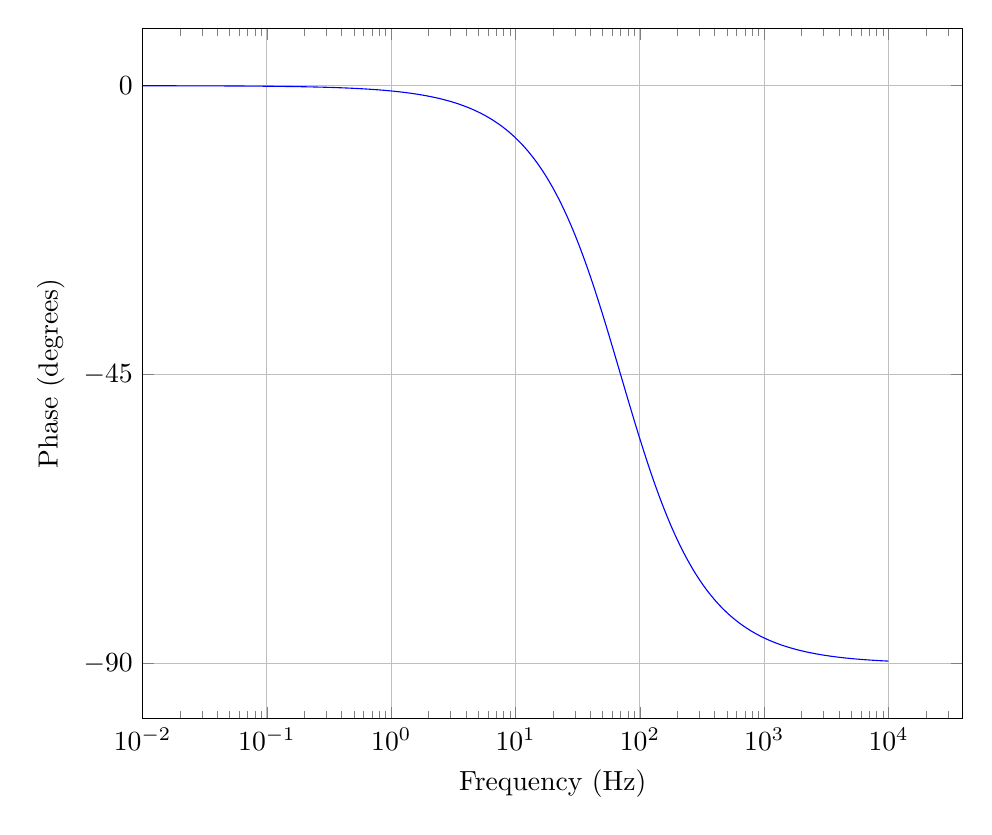
\begin{tikzpicture}
                    \begin{semilogxaxis}[
                        width=12cm,
                        xmin = 0.01,
                        xmajorgrids=true,
                        ymajorgrids=true,
                        xlabel={Frequency (Hz)},
                        ylabel={Phase (degrees)},
                        ytick={-180,-135,-90,-45,0,45,90,135,180},
                        yticklabels={$-180$,$-135$,$-90$,$-45$,$0$,$45$,$90$,$135$,$180$}
                    ] 
                        \addplot[domain=0.01:10000,samples=1000,color=blue]{(atan(-(x)/70))};
                    \end{semilogxaxis}
                \end{tikzpicture}
                \caption{Filtro elimina banda ideale fase}
                \label{fig:BS filter phase}
            \end{figure} 
            Tutti i filtri possono essere ricavati dal filtro \textbf{Low-Pass} \ref{Filtro Passa Basso di banda B - Low Pass Filter (LP)}
            o dal filtro \textbf{High-Pass} \ref{Filtro Passa Alto di banda B - High Pass Filter (HP)}.

            I filtri sono riconducibili a funzioni di trasferimento come quelle viste per il tracciamento di Bode nel corso
            di fondamenti di automatica.

            Sono giusti i grafici di bode? ricontrollare soprattutto la fase
        \subsubsection{Filtri non distorcenti}
            Definiamo prima cos'é  un sengale non distorto:
            \begin{figure}[H]
                \centering
                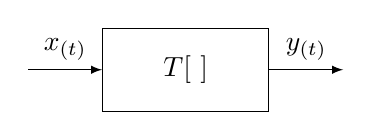
\begin{tikzpicture}[
                    node distance=2cm,
                    >=latex
                    ]
    
                    \node [coordinate] (input) {};
                    \node [draw, rectangle,right of = input, minimum height=3em, minimum width=6em] (block) {$T[\ ]$};
                    \node [coordinate, right of = block] (output) {};
                    
                    \draw[draw,->] (input) -- node[above]{$x_{(t)}$} (block);
                    \draw[->] (block) -- node[above]{$y_{(t)}$} (output);
                \end{tikzpicture}
                \label{fig:Sistema non distorcente}
            \end{figure}
            {\color{blue}$y_{(t)}$} é un segnale non distorto di $x$ se: $y_{(t)}\triangleq kx_{(t-t_0)}$ $k\in\mathbb{R}^+$, cioé finché esso rimane una versione
            ritardata e/o amplificata del segnale $x_{(t)}$, in frequenza:
            \[
                Y_{(f)} = kX_{(f)}e^{-j2\pi ft_0}   
            \]
            \begin{figure}[H]
                \centering
                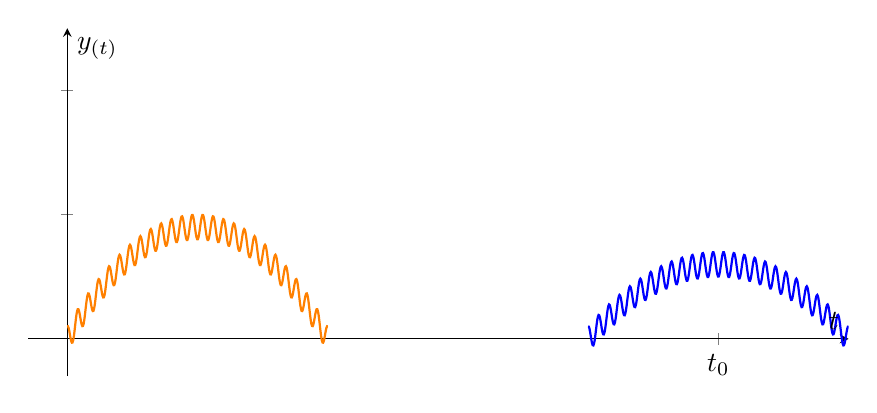
\begin{tikzpicture}
                    \begin{axis}[
                        domain=-0.3:15,
                        samples=200,
                        axis lines=middle,
                        xlabel=$t$,
                        ylabel=$y_{(t)}$,
                        xmax=6,
                        xmin=-0.3,
                        ymin=-0.3,
                        ymax=2.5,
                        xtick={5},
                        xticklabels={$t_0$},
                        ytick={},
                        yticklabels={},
                        width=12cm,
                        height=6cm
                    ]
                    \addplot [thick,orange, samples = 400, domain = 0:2] {-0.9*(x^2-2*x)+(0.1*cos(deg(25*x*pi)))};
                    \addplot [thick,blue, samples = 400, domain = 4:6] {-0.6*((x-4)*(x-6))+(0.1*cos(deg(25*x*pi)))};
                    
                    \end{axis}
                \end{tikzpicture}
                \label{fig:segnale non distorto}
            \end{figure} 
            

            \paragraph{Analisi del filtro non distorcente:}
            Come deve essere realizzato il filtro in modo tale da non distorcere il segnale?
            \[
                y_{(t)}=x_{(t)}\otimes h_{(t)} {\color{blue}=kx_{(t-t_0)}} 
            \]
            Per non essere distorcente la risposta impulsiva del sistema deve essere $k\delta_{(t-t_0)}$ con risposta in frequenza:
            $H_{(f)} = ke^{-j2\pi ft_0}$
            
            \begin{figure}[H]
                \centering
                \subfloat[Ampiezza con ritardo]{
                    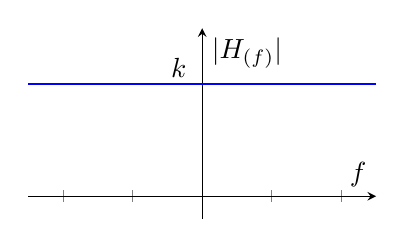
\begin{tikzpicture}
                        \begin{axis}[
                            domain=-5:5,
                            samples=200,
                            axis lines=middle,
                            xlabel=$f$,
                            ylabel=$|H_{(f)}|$,
                            ytick = {1},
                            yticklabels = {$k$},
                            xtick = {},
                            yticklabel style = {yshift=6pt}, 
                            xticklabels = {},
                            ymin=-0.2,
                            ymax=1.5,
                            width=6cm,
                            height=4cm
                        ]
                        \addplot [const plot,blue, thick] coordinates{(-5,1)(5,1)};
                        \end{axis}
                    \end{tikzpicture}
                    \label{fig:Ampiezza filtro non distorcente}
                }
                \hfill
                \subfloat[Fase con ritardo]{
                        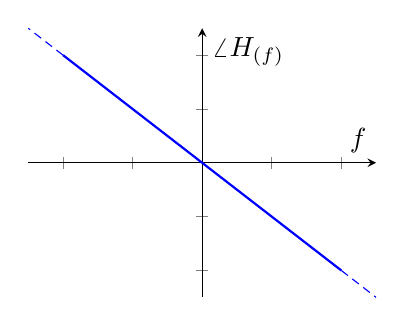
\begin{tikzpicture}
                            \begin{axis}[
                                domain=-5:5,
                                samples=200,
                                axis lines=middle,
                                xlabel=$f$,
                                ylabel=$\angle H_{(f)}$,
                                xmax=5,
                                xmin=-5,
                                xtick = {},
                                xticklabels = {},
                                ytick={},
                                yticklabel style = {yshift=6pt}, 
                                yticklabels={},
                                width=6cm,
                                height=5cm
                            ]
                            \addplot [blue, thick, samples = 300, domain = -4:4] {-x};
                            \addplot [blue, densely dashed] coordinates{(-4,4)(-5,5)};
                            \addplot [blue, densely dashed] coordinates{(4,-4)(5,-5)};
                            \end{axis}
                        \end{tikzpicture}
                    \label{fig:fase filtro non distorcente}
                }
                \caption{Spettro filtro non distorcente}
            \end{figure}
            Avere un tale filtro per tutti i segnali é molto restringente, ci basta che il nostro filtro sia non distorcente nella banda che ci interessa.
            
            \begin{figure}[H]
                \centering
                \subfloat[Ampiezza con ritardo]{
                    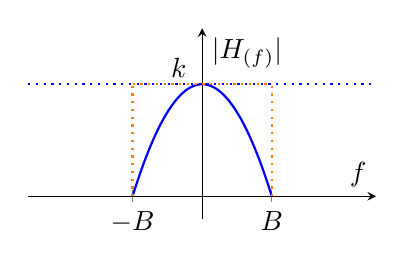
\begin{tikzpicture}
                        \begin{axis}[
                            domain=-5:5,
                            samples=1000,
                            axis lines=middle,
                            xlabel=$f$,
                            ylabel=$|H_{(f)}|$,
                            ytick = {1},
                            yticklabels = {$k$},
                            xtick = {-2,2},
                            yticklabel style = {yshift=6pt}, 
                            xticklabels = {$-B$,$B$},
                            ymin=-0.2,
                            ymax=1.5,
                            width=6cm,
                            height=4cm
                        ]
                        \addplot [dotted,blue, thick] coordinates{(-5,1)(5,1)};
                        \addplot [blue, thick, samples = 1000, restrict y to domain=0:1] {-(x/2)^2+1};
                        \addplot [dotted,orange, thick] coordinates{(-2,0)(-2,1)};
                        \addplot [dotted,orange, thick] coordinates{(2,0)(2,1)};
                        \addplot [dotted,orange, thick] coordinates{(-2,1)(2,1)};
                        \end{axis}
                    \end{tikzpicture}
                    \label{fig:Ampiezza filtro non distorcentein banda}
                }
                \hfill
                \subfloat[Fase con ritardo]{
                        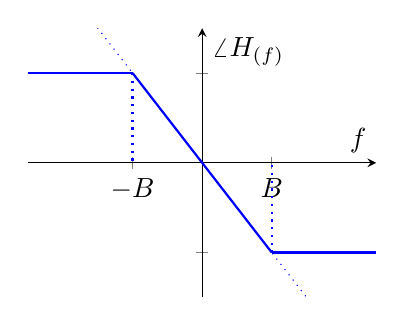
\begin{tikzpicture}
                            \begin{axis}[
                                domain=-5:5,
                                samples=200,
                                axis lines=middle,
                                xlabel=$f$,
                                ylabel=$\angle H_{(f)}$,
                                xmax=5,
                                xmin=-5,
                                ymin=-3,
                                ymax=3,
                                xtick = {-2,2},
                                xticklabels = {$-B$,$B$},
                                ytick={},
                                yticklabel style = {yshift=6pt}, 
                                yticklabels={},
                                width=6cm,
                                height=5cm
                            ]
                            \addplot [blue, dotted, samples = 300, domain = -5:5] {-x};
                            \addplot [blue, thick, samples = 300, domain = -2:2] {-x};
                            \addplot [blue, thick] coordinates{(-2,2)(-5,2)};
                            \addplot [blue, dotted,thick] coordinates{(-2,2)(-2,0)};
                            \addplot [blue, thick] coordinates{(2,-2)(5,-2)};
                            \addplot [blue, dotted,thick] coordinates{(2,-2)(2,0)};
                            \end{axis}
                        \end{tikzpicture}
                    \label{fig:fase filtro non distorcente in banda}
                }
                \caption{Spettro filtro non distorcente limitato alla banda $B$}
            \end{figure}            
            Il filtro ci basta che sia qualcosa che si avvicini a una $rect$ ad esempio un coseno rialzato \ref{F. Coseno Rialzato}

    \subsection{Th. di Parseval}\label{Th. di Parseval}
        \[
              E_{x} = \int_{-\infty}^{\infty}|x_{(t)}|^2 dt = \int_{-\infty}^{\infty}|X_{(f)}|^2 df =\int_{-\infty}^{\infty} S_{x(f)} df
        \]
        $S_{x(f)} = |X_{(f)}|^2$ é la densitá spettrale di energia del segnale, ci mostra come l'energia é distribuita nello spettro.
        
        Dimostrazione:
        \begin{align}
            E_{x} &= \int_{-\infty}^{\infty}|x_{(t)}|^2 dt =\int_{-\infty}^{\infty}x_{(t)}x_{(t)}^{\star} dt = \int_{-\infty}^{\infty}x_{(t)}\left[\int_{-\infty}^{\infty}X_{(f)}e^{j2\pi ft}df\right]^\star dt\nonumber \\
                  &= \underset{(t)}{\int_{-\infty}^{\infty}}x_{(t)}\underset{(f)}{\int_{-\infty}^{\infty}}X_{(f)}^\star e^{-j2\pi ft}dfdt = \underset{(f)}{\int_{-\infty}^{\infty}}X_{(f)}^\star\underset{(t)}{\int_{-\infty}^{\infty}}x_{(t)} e^{-j2\pi ft}dtdf \nonumber \\
                  &= \int_{-\infty}^{\infty}X_{(f)}^\star X_{(f)} df = \int_{-\infty}^{\infty}|X_{(f)}|^2 df\nonumber
        \end{align}
        Come capisco quanta \% del segnale sto buttando?

        \begin{figure}[H]
            \centering
            \begin{tikzpicture}
                \begin{axis}[
                    domain=-3:3,
                    samples=1000,
                    axis lines=middle,
                    xlabel=$f$,
                    ylabel=$|S_{x(f)}|$,
                    ytick = {},
                    yticklabels = {},
                    xtick = {-1.3,1.3},
                    yticklabel style = {yshift=6pt}, 
                    xticklabels = {$-B$,$B$},
                    ymin=-0.2,
                    ymax=1.5,
                    width=6cm,
                    height=4cm
                ]
                \addplot [blue, thick] {exp(-x^2)};
                \addplot [name path = A,domain=-3:-1.3,blue, thick] {exp(-x^2)};
                \addplot [name path = B,domain=1.3:3,blue, thick] {exp(-x^2)};
                \addplot [dotted,blue,thick] coordinates{(-1.3,0)(-1.3,0.15)};
                \addplot [dotted,blue,thick] coordinates{(1.3,0)(1.3,0.15)};
                \addplot [const plot,name path = C,black, thin] coordinates{(-1.3,0)(-3,0)};
                \addplot [const plot,name path = D,black, thin] coordinates{(1.3,0)(3,0)};

                \addplot[green,opacity = 0.5] fill between[of=A and C];
                \addplot[green,opacity = 0.5] fill between[of=B and D];

                \end{axis}
            \end{tikzpicture}
            \caption{Spettro $S_{x(f)}$}
        \end{figure}            
        \noindent La parte {\color{green}verde} é l'energia del segnale che perdiamo troncandolo con banda $B$
    \subsection{Funzione di Correlazione - Segnali Aperiodici}\label{Funzione di Correlazione - Segnali Aperiodici}
        \[
            C_{xy} = R_{xy(\tau)}=\int_{-\infty}^{\infty}x_{(t)}y_{(t-\tau)}^\star dt 
        \]
    \subsection{Funzione di Autocorrelazione}\label{Funzione di Autocorrelazione}
        \[
            C_x = R_{x(\tau)}=\int_{-\infty}^{\infty}x_{(t)}x_{(t-\tau)}^\star dt 
        \]
        \noindent Misura la correlazione del segnale con se stesso.
        \subsubsection{Propietá Autocorrelazione}
            \begin{itemize}
                \item {$R_{x(0)} = E_x$
                    \[
                        R_{x(0)} =\int_{-\infty}^{\infty}x_{(t)}x_{(t)}^\star dt =\int_{-\infty}^{\infty}|x_{(t)}|^2 dt = E_x   
                    \]
                }
                \item {Simmetria Hermitiana:
                    \[
                        R_{x(-\tau)} =R_{x(\tau)}^\star 
                    \]
                }
                \item {$TCF$ Autocorrelazione:
                    \[ 
                        R_{x(\tau)} \overunderset{TCF}{ATCF}{\rightleftharpoons} S_{x(f)}
                    \]
                    Posso calcolare la densitá spettrale di energia dall'autocorrelazione.
                }
            \end{itemize}